\section{Geometric interpretation}
Here is a geometric interpretation of the Grover algorithm, following from the observation that the quantum state~\ref{eq:initial-state} stays in a two-dimensional subspace after each step of the algorithm. We will show that the Grover iteration can be regarded as a rotation in the two-dimensional subspace spanned by the startinc vector $\ket{\psi}$ and the state $\ket{\beta}$ consisting of a uniform superposition of solutions to the search problem. 

We shall adopt the convection that $\sum_{x}^{''}$ indicates a sum over all $x$ which are solutions to the search problem, and $\sum_{x}^{'}$ indicates a sum over all $x$ which are note solutions to the search problem. Define normalized states.

\begin{equation*}
\begin{split}
 \ket{\alpha} &\equiv \frac{1}{\sqrt{N-M}} \sum_{x}{}^{''} \ket{x} \\
 \ket{\beta} &\equiv \frac{1}{\sqrt{M}} \sum_{x}{}^{'} \ket{x}
\end{split}
\end{equation*}
the initial state $\ket{\psi}$ may be expressed as:
\begin{equation*}
    \ket{\psi} = \sqrt{\frac{N-M}{N}} \ket{\alpha} + \sqrt{\frac{M}{N}} \ket{\beta}
\end{equation*}

Consider the subspace spanned by $\ket{\psi}$ and $\ket{\beta}$ and equivalently the subspace spanned by $\ket{\beta}$ and the orthogonal state $\ket{\alpha}$.
The algorithm begins with the initial ket $\ket{\psi}$, which lies in the subspace. The operator $\hat{U}_\beta$ is a reflection at the hyperplane orthogonal to $\ket{\beta}$ for vectors in the subspace spanned by $\ket{\alpha}$ and $\ket{\beta}$. This can be seen by writing $\hat{U}_\beta$ in the form of a Householder reflection\footnote{A Householder reflection is a linear transformation that describes a reflection about a plane or hyperplane containing the origin.}:

\begin{equation}
    \hat{U}_\beta = \hat{I} - 2 \ket{\beta}\bra{\beta}
\end{equation}
 The operator $\hat{U}_\psi = 2 \ket{\psi}\bra{\psi} - \hat{I}$ is a reflection through $\ket{\psi}$. Both operators $\ket{U}_\psi$ and $\ket{U}_\beta$ take states in the subspace spanned by $\ket{\alpha}$ and $\ket{\beta}$ to states in the subspace. The product of two reflections is a rotation. Therefore, the state space stays in this subspace for the entire algorithm (i.e. $G^k\ket{\psi}$ remains in the subspace spanned by $\ket{\alpha}$ and $\ket{\beta}$ for all $k$). 
 
 Let $\cos\theta/2 = \sqrt{(N-M)/N}$ so that $\ket{\psi} = \cos\theta/2\ket{\alpha} + \sin\theta/2\ket{\beta}$.  The effect of the two refelction is
 
 \begin{equation*}
    \hat{G}\ket{\psi} = \cos\frac{3\theta}{2} \ket{\alpha} + \sin\frac{3\theta}{2} \ket{\beta}
\end{equation*}

so the rotation angle is in fact $\theta$. It follows that continued application of $G$ takes the state to:
\begin{equation*}
    \hat{G}^{k}\ket{\psi} = \cos\biggl(\frac{2k+1}{2}\theta\biggr) \ket{\alpha} + \sin\biggl(\frac{2k+1}{2}\theta\biggr) \ket{\beta}
\end{equation*}

\begin{figure}
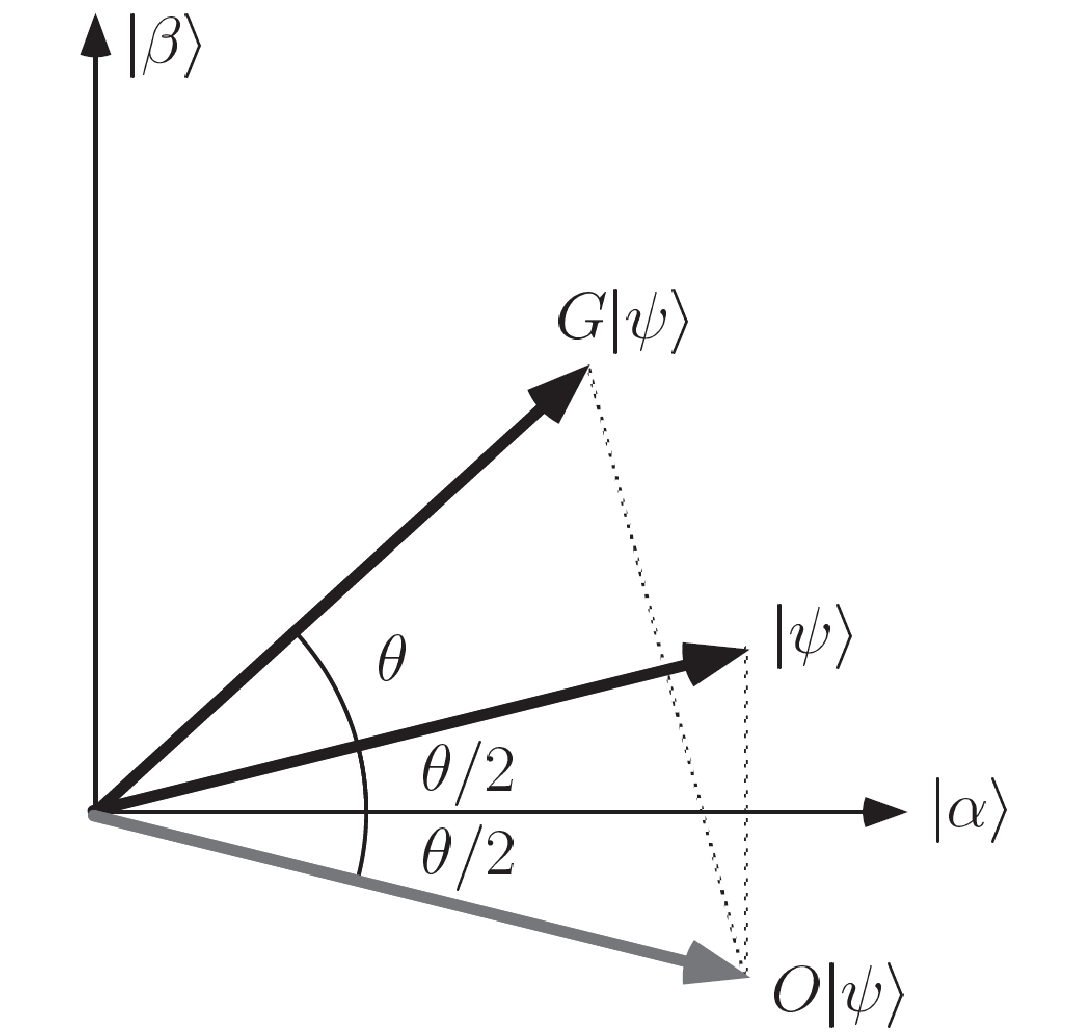
\includegraphics{geometric-interpretation.png}
\centering
\caption{The geometric interpretation of the first iteration of Grover's algorithm.}
\label{fig:geometric-interpretation}
\end{figure}

Repeated application of the Grover iteration rotates the state vector close to $\ket{\beta}$ as~\ref{fig:geometric-interpretation} shows.. When this occurs, an observation in the computational basis produces with high probability one of the outcomes superposed in $\ket{\beta}$, which is the solution.

